\chapter{Long Term Evolution for Railways (LTE-R)}
\label{chapter4}

This chapter provides background information on LTE proposed for high-speed railway communication system. It outlines the architecture for LTE-R leveraging the existing LTE network for high speed railway networks. For uniform coverage inside a tunnel environment, leaky coaxial cables (LCX) has been proposed for efficient communication. We explain LCX cables in details in the following chapter especially for tunnel environment. The severe channel impairments inside a tunnel are also discussed with special attention to high Doppler shift cause due to high velocities of trains and harsh multipath fading environment. Finally, the proposed two-ray propagation channel model is discussed and dynamic K-factor is derived.

\section{LTE-R Communication System}

In recent years, the use of trains have witnessed tremendous growth due to their increasing speeds, which has led to the demand for reliable wireless communication systems with these transportation systems. The development of a reliable wireless network for high speed trains is not a simple task and it is still an emerging technology. Global System for Mobile
Communication (GSM-R)~\cite{trlter1}, was a wireless communications standard designed for high speed trains, but it turned out not to be reliable enough and possess several limitations. The data rate of voice services which can reach up to 9.6 kbps, which can't meet the increasing demands of high-rate data transmission in railways communication. The limited data rate and quality of service (QoS) is not enough to support cellular communication for current generation. These reasons have made the evolution of high speed railway communication more and more urgent.  Subsequently, LTE~\cite{trlter2} proposed a promising solution for achieving broadband data rates, flexible bandwidth allocation and high spectral efficiency in high speed trains that can overcome various GSM-R limitations~\cite{arlter3,inplter4}.

\begin{figure}[!ht]
\centering
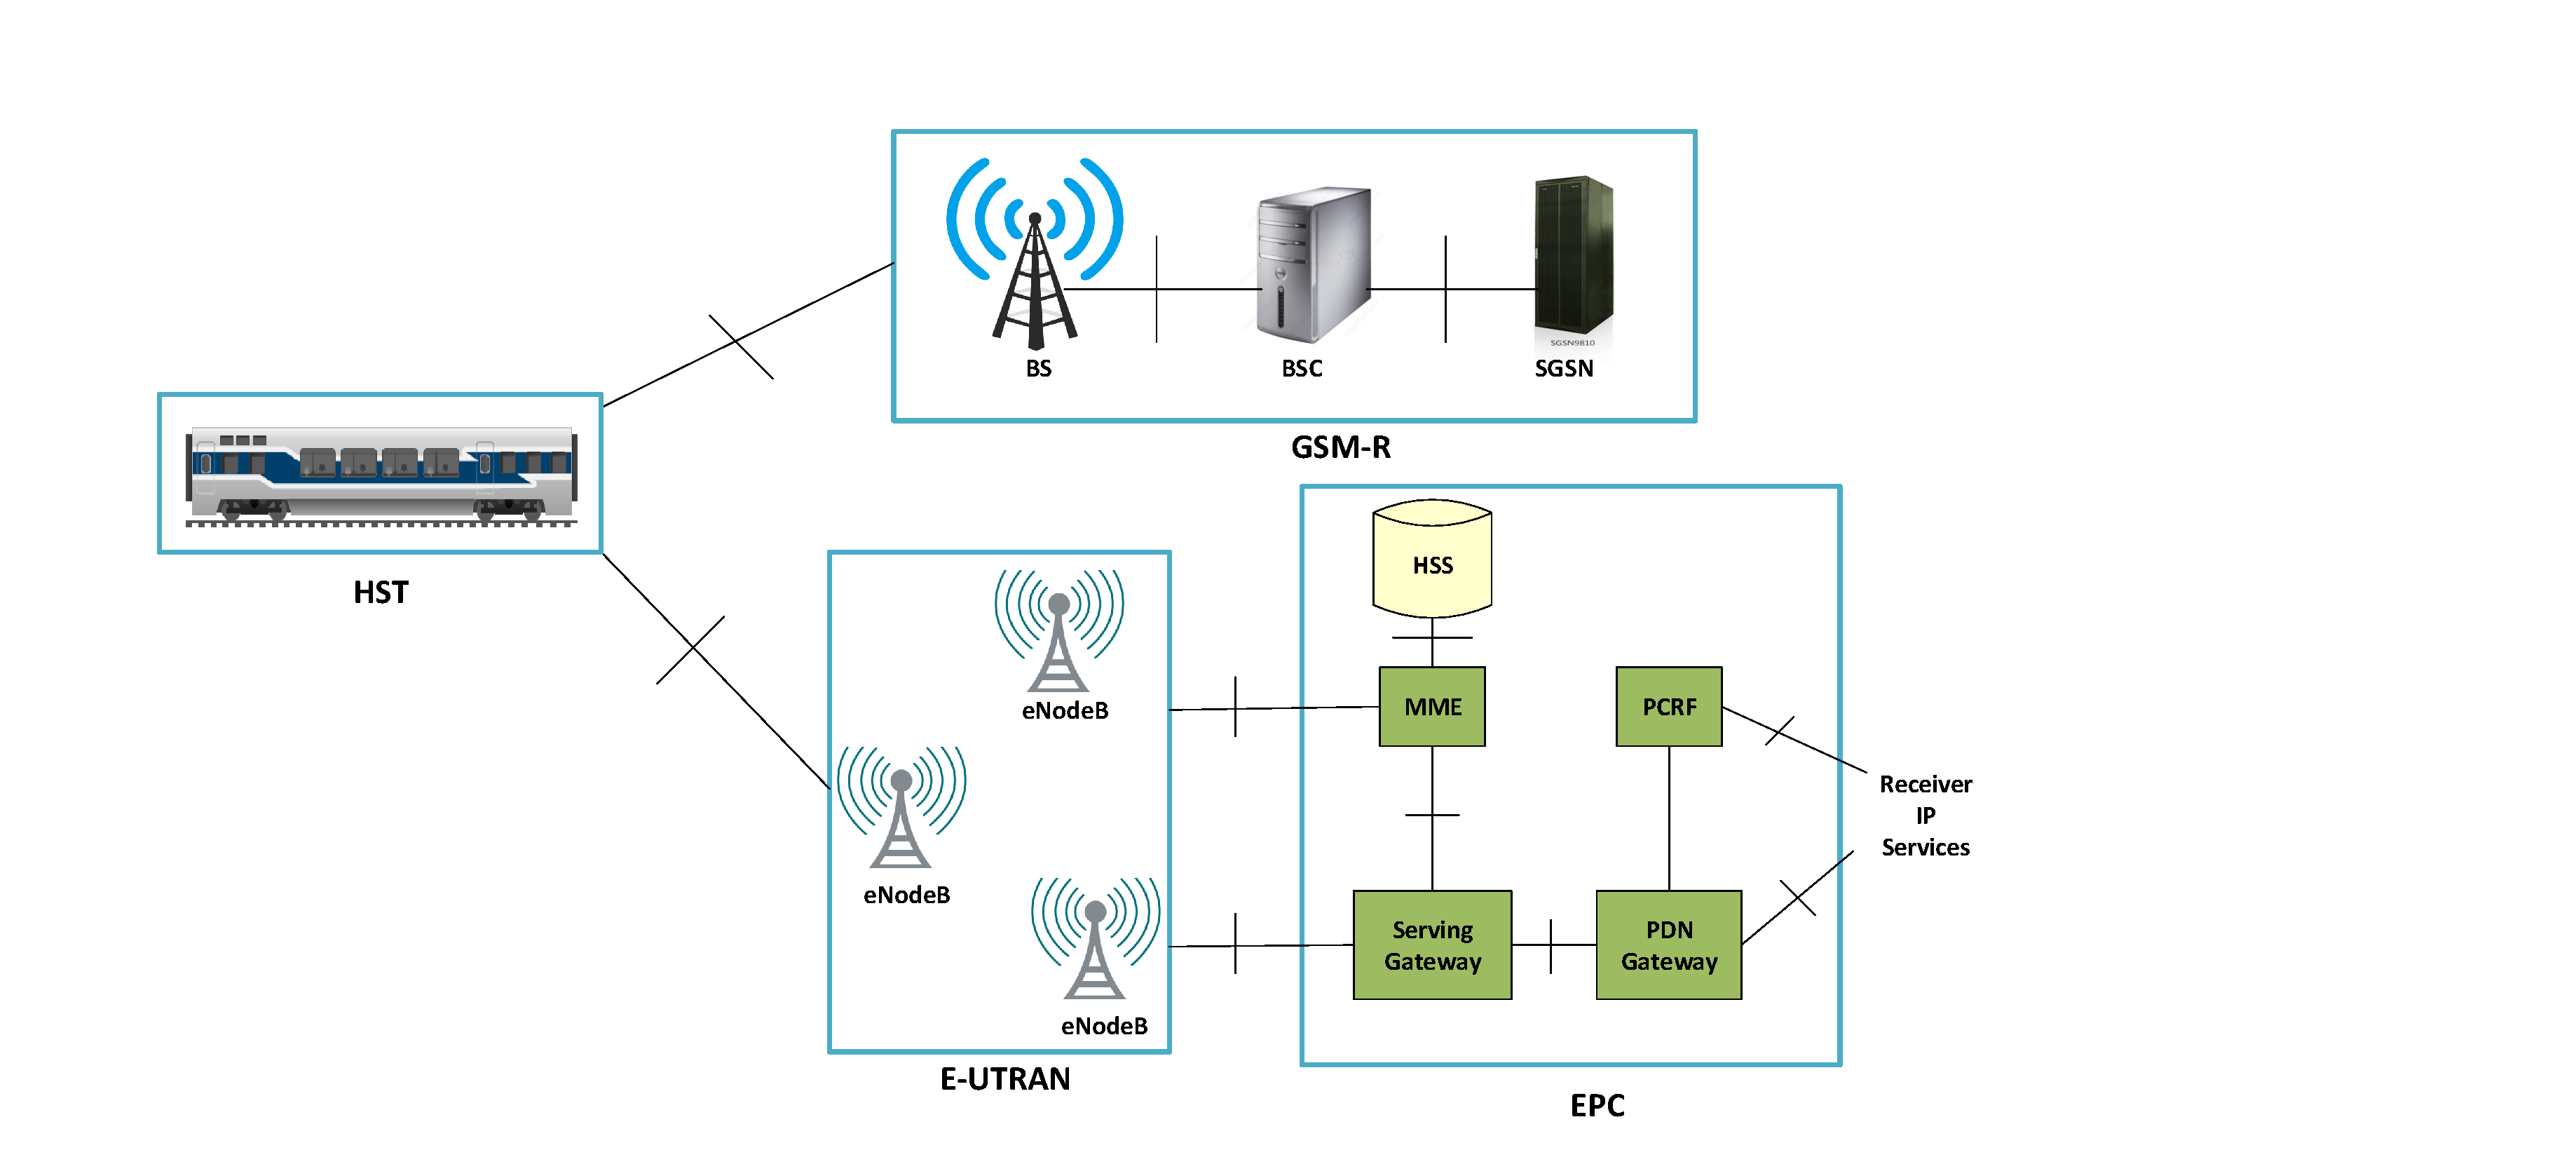
\includegraphics[width=\textwidth,keepaspectratio]{images/Gill/lte_figs/lter_architecture.eps} 
\caption{Proposed LTE-R Architecture for next generation High-speed Railways consisting of EPA and E-UTRAN.}
\label{ltearch}
\end{figure}

LTE-R is a high speed communication standard based on the existing LTE system architecture~\cite{inplter4}. There has been several studies regarding the assessment of LTE-R as a viable choice for next generation high speed communications for railway applications{inplter5,inplter6}. Conventional LTE includes a core network of evolved packet core (EPC) and a radio access network of Evolved Universal  Terrestrial  Radio  Access  Network (E-UTRAN). The  Internet  protocol (IP)-based  EPC  supports  seamless handovers for both voice and data to cell towers, and each E-UTRAN cell will support high data and voice capacity by high-speed  packet  access  (HSPA).  As  a  candidate for the next-generation  communication  system  of  HSR,  LTE-R  inherits all the important features of LTE and provides an extra radio access system to exchange wireless signals with onboard  units (OBUs)  and to match HST-specific  needs. Figure~\ref{ltearch} shows the proposed architecture of LTE-R according to~\cite{trlter2}, and it shows that the core network of LTE-R is backward compatible with GSM-R. The network architecture of LTE-R is similar to that of LTE/SAE with  Evolved Universal Terrestrial Radio Access Network (E-UTRAN) being the access network structure of LTE-R. There is evolved-Node B (eNodeB) that communicates directly with UEs like base transceiver station (BTS) in GSM network. It performs the transmission and reception of data packets using orthogonal frequency division multiplexing access (OFDM) for downlink and single carrier  frequency division multiple access (SC-FDMA) for uplink at PHY layer. At the same time, as without base-station controller (BSC), it also has functions of  radio  resource  control and wireless  mobility  management.  The eNodeBs can be connected to network router directly without more intermediate control nodes, such as the BSC in GSM-R~\cite{tingting2010high}. The core network of LTE-R is the Evolved Packet Core (EPC). The significant difference between EPC and the core network of GSM-R is that the EPC is an all-IP mobile core network.

\begin{table}[h!]
\caption{Comparison of system parameters between GSM-R , LTE and LTE-R.}
\begin{adjustbox}{width=1.22\textwidth, center=\textwidth}
\begin{tabular}{c | c | c | c}
\toprule
System Parameters & GSM-R & LTE & LTE-R\\ 
\midrule
Frequency & \shortstack{Uplink: 876--880 MHz\\downlink: 921--925 MHz} & 800, 1800, 2600 MHz & 450, 800, 1400, 1800 MHz \\  
Capacity  & 0.2 MHz & 1.4-20 MHz & 1.4-20 MHz\\ 
Modulation  & GMSK & QPSK/16-QAM/64-QAM & QPSK/16-QAM\\ 
MIMO  & No  & 2x2, 4x4  & 2x2\\ 
Cell Range  & 8 Km  & 1-5 Km & 4-12 Km \\ 
Data Rates (DL/UL)  & 172/172 Kbps  & 100/50 Mbps & 50/10 Mbps\\ 
\bottomrule
\end{tabular}
\end{adjustbox}
\label{ltertable}
\end{table}

Conventional LTE networks are different compared to LTE-R in many ways such as architecture, system parameters, network layout, services and quality of service (QoS). Table~\ref{ltertable} summarizes the LTE-R parameters and describe the differences between LTE, GSM-R and LTE-R. Since the LTE-R environment has very severe fading and high Doppler shift, it is configured for QoS rather than higher data rates. Therefore, QPSK modulation is used for most number of subcarriers and the number of packet re-transmission must be kept low and achieved with user datagram protocol (UDP).

\section{Leaky Coaxial Cable for LTE-R}
Leaky Coaxial Cable (LCX)~\cite{n1974leaky} is an antenna technology designed to deliver radio services in tunnel environment. It consists of small periodic slots to allow radio frequency (RF) signals to escape which act as extended antenna elements. LCX cables were invented to provide the uniform signal coverage in underground mine where radio coverage was very limited due to the geography of the mines. Recently, leaky coaxial cables have been widely used in the field of railway communication especially in tunnels. Leaky feeders are
constructed from coaxial cable where the outer shield has a series of holes with different shapes and different distances among them. The coaxial cable is usually about hundreds of metres long and can be fixed through a building or a tunnel offering radio radiation in a way that would require many individual omni-directional antennae. So far,they have been only used to supplement the direct wireless communication system between a BS and trains, mostly transmitting voice signals. Nowadays, they are being used as an alternative solution to distributed antenna systems in indoor environments like commercial buildings~\cite{motley1983directed,saleh1987distributed} and university buildings, high speed trains, cars, etc. The LCX radio system is almost noise free and has enough bandwidth to support multiple RF signals carrying voice and data simultaneously. Figure~\ref{fig:leakcoax} shows the conventional leaky coaxial cable along x-axis with periodic radiating slots and wave propagation along z-axis. Generally, it consists of three parts: inner conductor, dielectric material and inner conductor. LCX has a dual functionality i.e. they can transmit and receive RF signals using their slots. The frequency range for a leaky cable is given by~\cite{cao1999radio}:
\begin{equation}
\dfrac{c}{\sqrt{\varepsilon_r-1)}d}\geq f \leq \dfrac{c}{\sqrt{\varepsilon_r}+1)d}
\end{equation}

\begin{figure}[!ht]
\label{fig:leakcoax}
\centering
\includegraphics[width=\textwidth,keepaspectratio]{images/Gill/lte_figs/leakycoax.eps} 
\caption{Leaky Coaxial Cable}
\end{figure}

A radio system based on LCX has been deployed in Japan for high speed railways ''Series N700''~\cite{takatsu2007history} to connect the train to ground network. Wi-Fi access points are chosen for in-train communications with peak data rates of 2 Mbps for uplink and downlink. Although current technologies can provide wireless communication services in HSTs, the capacity of communication system is very low (1--4 Mbps). These data rates are insufficient for next generation wireless communication system where the peak data rates of 0.5 -- 5 Gbps are expected. LTE-R communication system can be implemented for achieving high data rates but it cannot be achieved by using conventional cellular system. The penetration loss due to tunnel walls is very high and secondly, the fast moving trains causes large Doppler shifts leading to poor connectivity due to retransmissions. Hence, leaky coaxial cable is the best candidate for achieving extensive internet access inside a tunnel environment for high speed railways.

\section{Channel Impairements Inside a Tunnel}
The tunnel environment is affected by multipath and diffraction effects due to multiple reflections from the tunnel walls, which leads to a substantial fading environment. By deploying LCX cables, we can eliminate the large penetration loss due to tunnel walls. However, small-scale fading can still cause a large amount of errors and decrease the QoS for the communication link. High velocity trains experience very high Doppler shifts and a fast fading channel. These problems can lead to significant BER degradation of the LTE system. The frequency shifts caused by the Doppler phenomenon can lead to shifts in the sub-carrier frequencies for OFDM, which leads to synchronization errors. The maximum Doppler shifts for a train traveling at 500 km/h is 2.314 kHz for a 5 GHz carrier frequency. This large Doppler shift can also lead to significant drops in the quality of wireless signals and increase the bit error rate. Thus,
to develop an efficient and reliable communication link inside tunnels, we need to properly model this channel impairment and build our proposed channel model by taking into account these tunnel phenomenons. These impairments are described in detail in the following subsections.

\subsection{Multipath Fading}
The following time-varying multipath channel impulse response considers the effects of Doppler shift and scattering~\cite{booklter13}:
\begin{equation}
\label{channel}
{h}(\tau,t)= \sum_{k=0}^{L}{h_k}(t)e^{-j2\pi f_c\tau_k(t)}\delta[\tau-\tau_k(t)],
\end{equation}
where $\tau$ is the path delay, $t$ is time in seconds, $\delta[\tau-\tau_k(t)]$ is the impulse response, $f_c$ is the carrier frequency, $h_k(t)$ is the envelope of the time-varying channel and consists of both large and small-scale fading components. Since the structure of LCX is almost the same as a leaky waveguide, the large scale fading of channel can be modeled linearly~\cite{arlter10}. There is also no signal shadowing and the line-of-sight (LOS) signal component is always present along the tunnel. This type of channel fading can be best described by a Ricean fading model. The probability density function $p(\alpha)$ of a Rician fading model is given by~\cite{inplter12}:
\begin{equation}
p(\alpha) = \dfrac{2\alpha(1+K)}{\Omega}I_0\Bigg(2\alpha\sqrt{\dfrac{K+K^2}{\Omega}}\Bigg)e^{\dfrac{-K-\alpha^2(1+K)}{\Omega}},
\end{equation}
where $K$ is the Rician factor and $\alpha$ is the complex amplitude of the channel response function that has a unity second moment, \textit{i.e.}, $\Omega \equiv E[\alpha^2] = 1$.

\subsection{Doppler Shift}
The 3GPP channel model~\cite{trlter14} is used for its Doppler shift profile in high speed railway environment. The measurements obtained for the Doppler frequency shift are implemented for two scenarios. The first scenario is for an open space while the second scenario is for high speed trains. Doppler shift is not taken into consideration. There exists a third scenario for tunnels using multiple antennas. Since the slots of LCX can be modeled as multiple antenna system, we use this Doppler shift profile for our proposed channel. The Doppler shift variation $f_s(t)$ is described by:

\begin{equation}
\label{eq1}
f_s(t) = f_d\cos\theta(t),
\end{equation}
where \textrm{$f_d$} is the maximum Doppler shift, $\theta$ is the elevation angle and $\cos \theta(t)$ is given by:
\begin{equation}
\cos\theta(t) = 
\left\{
	\begin{aligned}
	 & \dfrac{D_s/2-vt}{\sqrt{\mathrm{D_{min}}^2+\bigg((D_s/2)-vt\bigg)^2}},0\leq t\leq\dfrac{D_s}{v}\\
	 & \dfrac{-1.5D_s+vt}{\sqrt{\mathrm{D_{min}}^2+\bigg((-1.5D_s)-vt\bigg)^2}},\dfrac{D_s}{v}\leq t \leq \dfrac{2D_s}{v}\\
 	\end{aligned}
\right.
\end{equation}
where $D_s/2$ is the initial distance of the train from base-station, and $\mathrm{D_{min}}$ is base-station (BS)-Railway track distance, both in meters; $v$ is the velocity of the train in \textrm{m/s}, $t$ is time in seconds.

\begin{figure}[!ht]
\label{doppler}
\centering
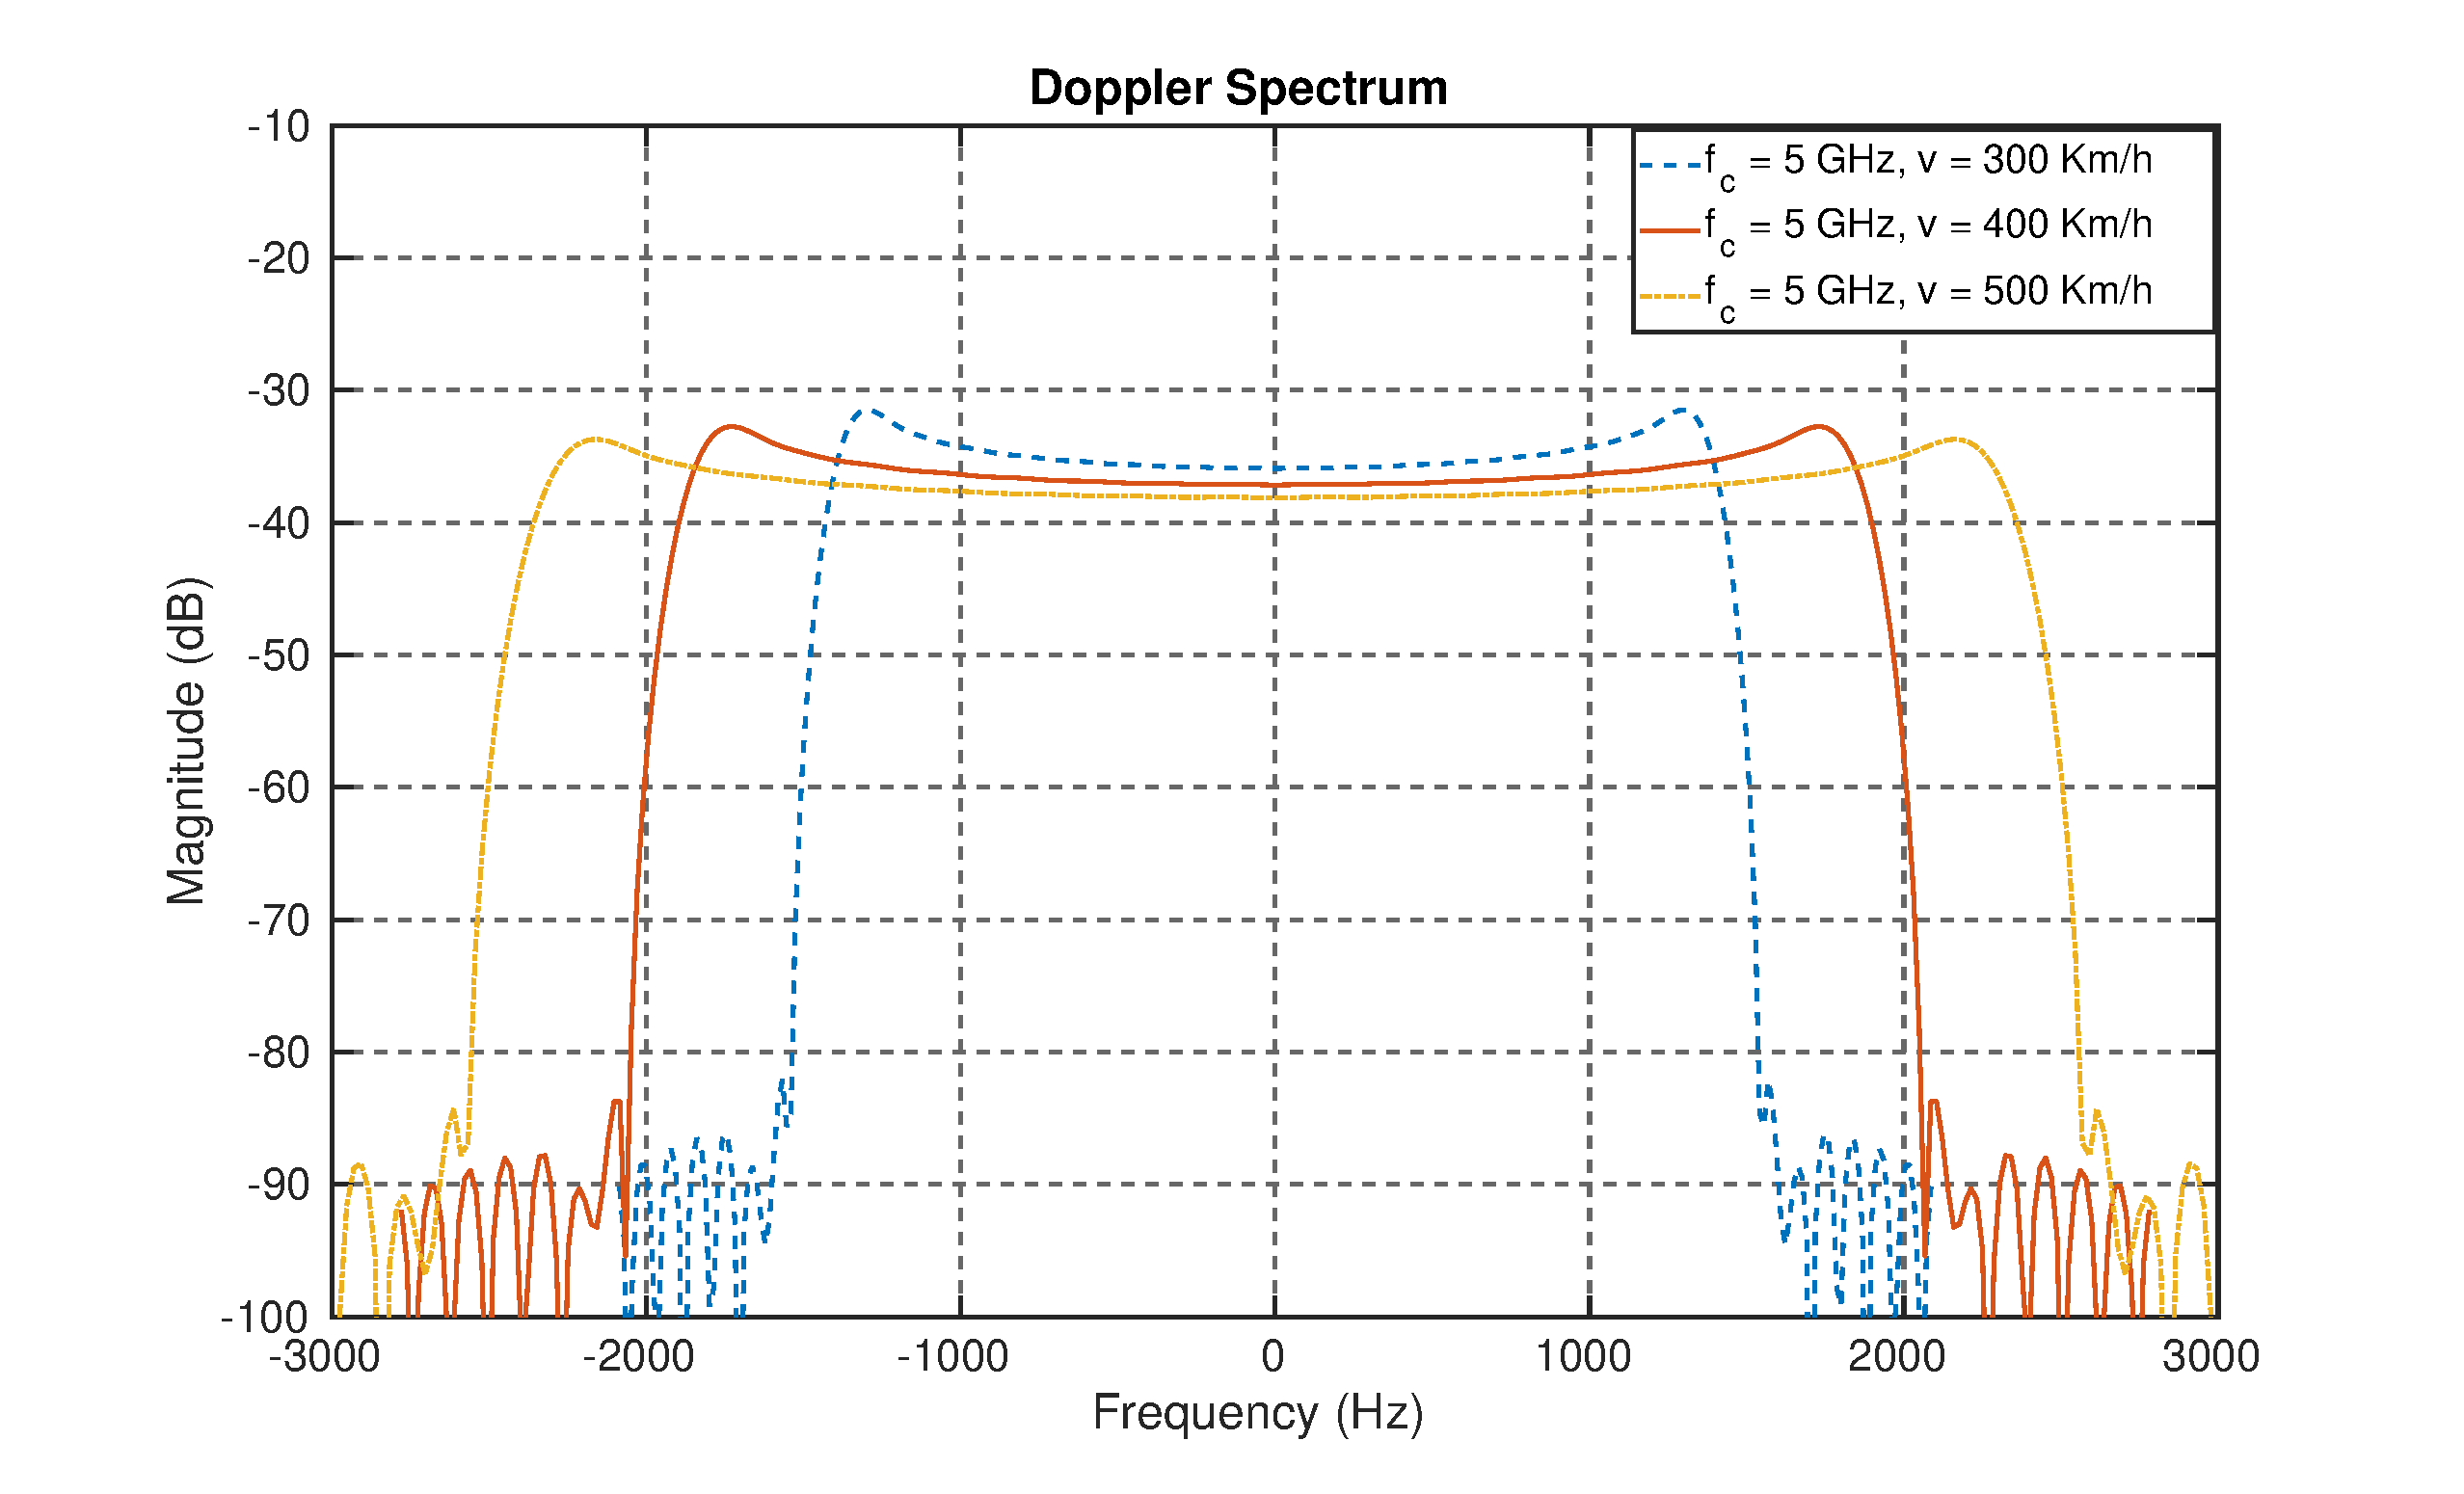
\includegraphics[width=\textwidth,keepaspectratio]{images/Gill/lte_figs/dopplerspectrum.eps} 
\caption{Doppler spectrum for LTE-R at different train velocities $v$ (km/h) = 300, 400 and 500 and $f_c$ = 5 GHz.}
\end{figure}

Figure~\ref{doppler} shows the Doppler spectrum for $f_c$ = 5 GHz and $v$ = 300 Km/h, 400 Km/h and 500 Km/h, and as we can see in the figure the maximum Doppler shift range is from -2.314 kHz to +2.314 kHz. These range of Doppler shift values can lead to very high bit-error rate and poor connectivity in communication system. In the following section we discuss our proposed channel model which consists of Doppler shift profile for high speed train and dynamic K-factor for tunnel environment.

\section{Proposed Channel Model}

The tunnel measurement campaign conducted in~\cite{inplter8} shows that the amplitude variation inside tunnel follows Rician distribution. In the thesis, we apply the approach used in~\cite{inlter15} for single elevation angle $\theta$ and expand it to a time-varying case. In this thesis, we model $\theta$ as a function of time and derive time-series $K$-factor for the tunnel environment. Figure~\ref{subblock} describes our proposed channel model which is implemented using dynamic K-factor and Doppler shift profile derived using Eq.(\ref{eq1}).  In the following section we discuss the classical two-ray propagation model and mathematical derivation of dynamic K-factor for our proposed channel model.

\begin{figure}[!ht]
\label{subblock}
\centering
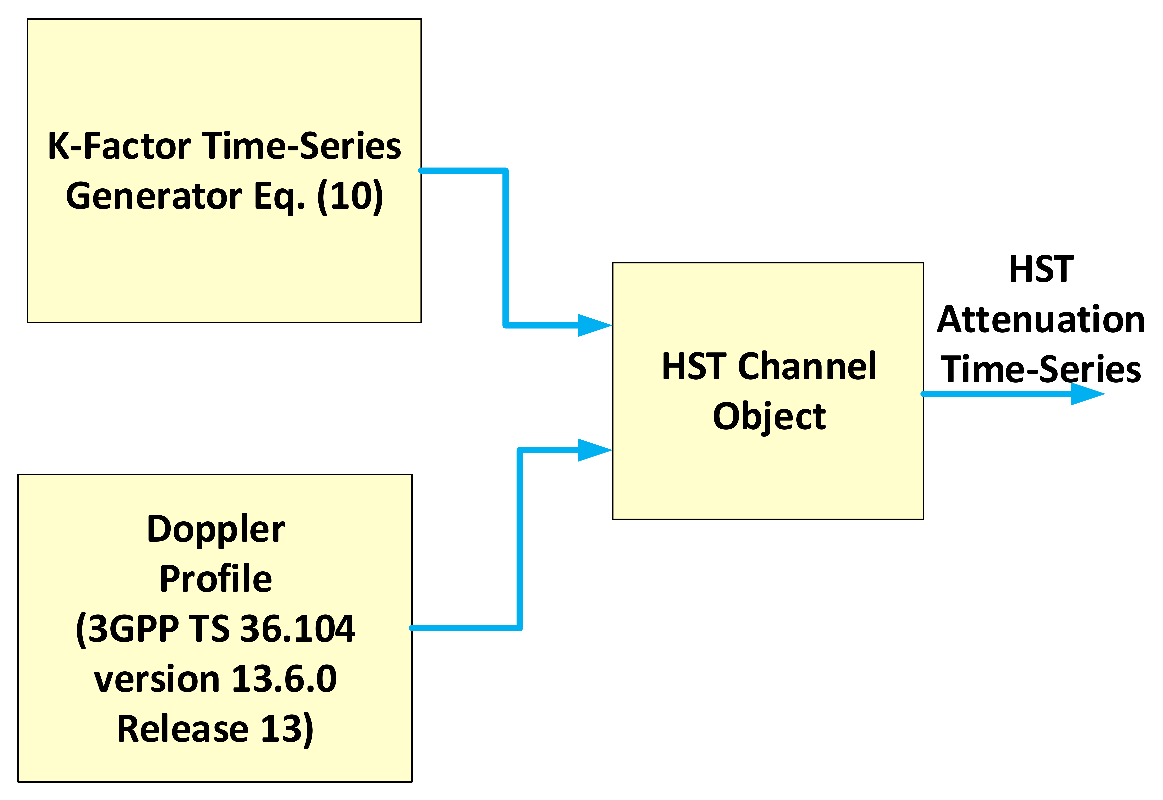
\includegraphics[width=\textwidth,height=6cm,keepaspectratio]{images/Gill/lte_figs/subblock.eps} 
\caption{HST channel model consisting of time-series K-factor and Doppler shift caused due to velocity of the train.}
\end{figure}

The reflection coefficient $\Gamma$~\cite{booklter16} as a function of time $t$ is given by:
\begin{equation}
\Gamma(t) = \dfrac{C\sin\theta(t)-\sqrt{(\varepsilon_r-j\chi(t))-(\cos\theta(t))^2}}{C\sin\theta(t)-\sqrt{(\varepsilon_r-j\chi(t))-(\cos\theta(t))^2}},
\end{equation}
where $C = 1$ is for horizontal polarization, and $C = \varepsilon_r-j\chi(t)$ for vertical polarization. Furthermore, $\chi(t)$ is given by:
\begin{equation}
\chi(t) = \dfrac{\sigma}{\omega(t)\varepsilon_0} = \dfrac{\sigma}{2\pi f_r(t) \varepsilon_0} = \dfrac{1.8\times 10^{10}\sigma}{f_r(t)}.
\end{equation}
with $\varepsilon_0 = 8.854\times 10^{-12}~\textrm{F/m}$, and $\sigma$ is conductivity of the tunnel. The frequency $f_r(t)$ is the resultant frequency caused by the Doppler shift and is given by:
\begin{equation}
f_r(t) = f_c(t)-f_s(t)
\end{equation}
where $f_c(t)$ is the sub-carrier frequency, and $f_s(t)$ is the Doppler shift given by Eq.~(\ref{eq1}).

The phase difference function of $t$, $\Delta\phi(t)$ between the two reflected paths is given by~\cite{booklter11}:
\begin{equation}
\begin{split}
\Delta\phi(t) =& \dfrac{2\pi}{\lambda(t)}\bigg(\sqrt{D_{\textrm{LOS}}^2+(h_t+h_r)^2}-\\
& \sqrt{D_{\textrm{LOS}}^2+(h_t-h_r)^2}\bigg),
\end{split}
\end{equation}
where $\lambda(t)$ is the resultant time-varying wavelength at the receiver, $D_{\textrm{LOS}}$ is the distance between the transmitter and receiver antennas which is changing dynamically with $t$, and both $h_t$ and $h_r$ are the heights of the transmitter and receiver antennas, respectively.
 
The resultant received power $p_r(t)$ is given by the sum of the LOS received power plus the received multipath power, resulting in:
\begin{equation}
\begin{split}
p_r(t) =& ~p_t(t)\bigg(\dfrac{\lambda}{4\pi d}\bigg)^2G_t G_r\bigg[1+\\
& |\Gamma(t)|^2+2|\Gamma(t)|\cos(\angle\Gamma(t)-\angle\Delta\phi(t))\bigg]
\end{split}
\end{equation}
which is a function of the transmitter power $p_t(t)$ and the reflection coefficient $\Gamma(t)$, where $G_t$ and $G_r$ are the transmitter and receiver antenna gains,  respectively.
The $K$-factor is defined as the ratio of the direct path power and the power in the scattered paths, and is given as:
\begin{equation}
\label{kfactor}
\mathrm{K}(t) = \dfrac{1}{|\Gamma(t)|^2+2|\Gamma(t)|\textrm{cos}(\angle \Gamma(t)-\Gamma(t)\Delta\Phi(t))}
\end{equation}

\section{Summary}
This chapter outlined and examined the topics of jamming and anti-jamming techniques, and provided a foundation in communication system theory and advanced equalizer design.  Secondly it setup an understanding of Software-Defined Radio, the power of such an architecture, and examples of implementations and existing software for future designs.  Next, this thesis will consider a new anti-jamming technique and design an implementation of such a system.  After the implementation is investigated, the result of specific experiments on such an implementation will be analyzed.\\
